% !Mode:: "TeX:UTF-8"

% 默认为本科生开题报告
% 如需修改为硕士/博士开题报告,请将bachelor替换为master/doctor
\documentclass[bachelor, ktreport, twoside, color]{buaathesis}
% openany, oneside
% 参考文献
\usepackage{gbt7714}
% 参考文献输出方式,numerical为按照出现顺序,authoryear为按照作者姓名和年份
\citestyle{numerical}
% \citestyle{authoryear}

\begin{document}

% 开题文件类型,如果为文献综述请自行更改
\ktclass{开题报告}

% 学院中英文名称
\school{(学院名)}{(Name of School)}

% 专业中英文名
\major{(专业名)}{(Name of Major)}

% 研究方向名称(仅研究生)
\direction{(研究方向)}

% 论文中英文标题(注意,无论是否有子标题,必须包含3个以上的大括号)
\thesistitle{北京航空航天大学学位论文\LaTeX{}模板}{}{}

% 学号
\studentID{(学号)}

% 作者中英文名
\thesisauthor{(姓名)}{(Name)}

% 导师中英文名
\teacher{(导师姓名)}{(Name of Tutor)}

% 毕设答辩时间
\thesisdate{(年)}{(月)}

% 页眉页脚样式
\pagestyle{mainmatter}

% 封面、任务书、声明
\maketitle

% 前言页眉页脚样式
\pagestyle{frontmatter}

% % 摘要,仅文献综述需要
% % !Mode:: "TeX:UTF-8"

% 中英文摘要
\begin{cabstract}
    许多用于小样本学习的元学习方法依赖于简单的基础学习器,例如最近邻分类器。
    然而,即使在少样本的情况下,经过区分训练的线性预测器也可以提供更好的泛化。
    我们建议使用这些预测器作为基础学习器来学习小样本学习的表示,
    并展示它们在一系列小样本识别基准中在特征大小和性能之间提供更好的权衡。
    我们的目标是学习在新类别的线性分类规则下可以很好地泛化的特征嵌入。
    为了有效地解决目标,我们利用了线性分类器的两个特性:
    凸问题最优条件的隐式微分和优化问题的对偶公式。
    这使我们能够在适度增加计算开销的情况下使用具有改进泛化的高维嵌入。
    我们的方法名为MetaOptNet,在miniImageNet、tieredImageNet、
    CIFAR-FS和FC100小样本学习基准上实现了最先进的性能。


\end{cabstract}

\begin{eabstract}
    Many meta-learning approaches for few-shot learning rely on 
    simple base learners such as nearest-neighbor classifiers.
     However, even in the few-shot regime, discriminatively trained linear predictors can offer better generalization. 
     We propose to use these predictors as base learners to learn representations for 
     few-shot learning and show they offer better tradeoffs between feature size and 
     performance across a range of few-shot recognition benchmarks. 
     Our objective is to learn feature embeddings that generalize well under a 
     linear classification rule for novel categories. To efficiently solve the objective, 
     we exploit two properties of linear classifiers: implicit differentiation of the optimality 
     conditions of the convex problem and the dual formulation of the optimization problem. 
     This allows us to use high-dimensional embeddings with improved generalization at a modest increase 
     in computational overhead. Our approach, named MetaOptNet, achieves state-of-the-art performance on 
     miniImageNet, tieredImageNet, CIFAR-FS, and FC100 few-shot learning benchmarks.
\end{eabstract}

% 目录
\tableofcontents

% 正文页码样式
\mainmatter
% 正文页眉页脚样式
\pagestyle{mainmatter}

% 正文


\chapter{绪论}

\section{课题研究背景}

从有限的例子中学习是人类智慧的特征,但它仍然是现代机器学习系统的挑战。这个问题引起了机器学习界的极大关注,在机器学习界,
只有少数几个例子的机器学习被认为是一个元学习问题。其目标是在只有少数训练数据的任务中最大限度的减少泛化误差。
典型的方法由一个将输入域映射到特征空间的嵌入模型和一个将特征空间映射到任务变量的基本学习器组成。元学习的目标是
学习一个嵌入模型,从而使基础学习器在不同的任务中具有良好的泛化能力。

\section{课题研究意义}

虽然目前存在许多基础学习器的选择,但最临近分类器以及其变体是最重要的。
由于分类规则简单,该方法在低数据系统中具有良好的扩展性,因此该方法很受欢迎。
然而在低数据情况下,经过鉴别训练的线性分类器的表现往往优于最临近分类器,因为他们能很好的利用反面例子,
通常更丰富,从而更好的学习类别的边界。
此外,他们可以通过适当的正则化,如权值系数性和或范数等,有效的利用高维特征嵌入来控制模型的容量。


\section{课题研究内容}




\chapter{模块2 (解决方案)}


\section{问题描述}

给定训练集 $D^{train} = \{(x_t,y_t)\}^{T}_{t=1}$ ,基学习器 $A$ 的目标是利用参数 $\theta$ 对预测器 $y=f(x,\theta)$ 进行估计,
以在未见的测试集 $D^{test} = \{(x_a, y_a)\}^{Q}_{t=1}$ 上实现更好的泛化能力,
通常假设训练集和测试集采样自相同分布,并使用参数 $\phi$的嵌入模型$f_{\phi}$将样本域映射到特征空间。
对于基于优化的学习器,参数通过最小化训练数据上的经验损失以及正则项(以鼓励模型的简洁性)获得。

\begin{equation}
    \theta = A(D^{train}; \phi) = argmin_{\theta}L^{base}(D^{train}; \theta, \phi) + R(\theta)
\end{equation}

其中,$L^{base}$ 是损失函数,$R(\theta)$ 是正则项,在训练数据有限的情况下,正则项在模型的泛化方面扮演很重要的角色。

为了最小化泛化误差,少样本元学习方法旨在学习任务分布中的最优模型,这可以看作是在一个任务集合上进行学习:
$T = \{(D_{i}^{train}, D_{i}^{test})\}^{I}_{i=1}$,通常被称为元训练集。
通过元组$(D_i^{train}, D_i^{test})$描述的训练和测试数据集,或任务,
我们的目标是学习一个嵌入模型$\phi$,使得在给定基础学习者$A$的情况下,在不同任务中达到最小化泛化(或测试)误差的效果。

为了实现这一目标,我们的学习目标是:

\begin{equation}
    \min_{\phi} E_{T} [L^{meta}(D^{test}; \theta, \phi), where \theta = A(D^{train}, \phi)]
\end{equation}

图1展示了单一任务的训练和测试过程。一旦学习到嵌入模型 $f_{\phi}$,它的泛化性能可以在一个保留的任务集合(通常称为元测试集)上进行评估。元测试集 
$S = \{(D_j^{train}, D_j^{test})\}^J_{j=1}$ 可以用公式来计算:

\begin{equation}
    E_S[L^{meta}(D^{test}; \theta, \phi), where \theta = A(D^{train}; \phi)]
\end{equation}

根据之前的研究,公式2和3中期望值的估计分别被称为元训练和元测试阶段。
在元训练阶段,我们会保留一个额外的验证集来选择元学习器的超参数并挑选最佳的嵌入模型。

\section{创新思想}
本文将可微的二次规划求解器和不同的线性分类器综合起来。利用以上两个特性,本文实现了在
计算成本略有增加的情况下提供了比最临近分类器更大的收益。

本文利用线性分类器的凸优化性质,将线性分类器作为基础学习器应用于元学习,用于解决可计算性问题。


\section{具体方法}
\subsection{任务集}
少样本学习使用K-way,N-shot分类任务对模型进行评估,
其中K表示类别数,$N$表示每个类别的训练样本数,通常取较小的值,
如$N\in{1,5}$。
虽然miniImageNet等数据集没有明确给出训练集和测试集$(D_i^{train}, D_i^{test})$,
但每个元学习任务可以在元训练阶段即兴构建,这被称为“episode”。
例如,一个episode $\tau_i=(D_i^{train}, D_i^{test})$ 可以按以下方式进行采样:

总体类集为$C^{train}$, 对于每个 episode,首先类$C_i$(包含来自$C^{train}$的K类)被有放回抽样得到,
然后训练集$D_i^{train} = \{(x_n, y_n) | n=1,...,N \times K, y_n \in C_i\}$(每个类包含N个图像)被采样;
最后测试集$D_i^{test} = \{(x_n, y_n) | n = 1,...,Q \times K, y_n \in C_i\}$(每个类包含Q个图像)被采样;

这里需要无放回抽样,如$D_i^{train} \cap D_i^{test} = \emptyset $,以优化泛化误差。以同样的方式从$C^{val}$
和$C^{test}$各自即兴构造元验证集(meta-validation)和元测试集(meta-test)。
为了度量嵌入模型对未见类的泛化,$C^{train}, C^{val}, C^{test}$需被互斥选择;

\subsection{凸基学习器}

当选择基学习器$A$时,必须考虑计算的效率,因为基学习器的计算效率直接影响到方程2中期望值的计算。
同时,在估计嵌入模型参数$\phi$时,也必须能够有效地计算任务测试误差$L^{meta}(D^{test}; \theta,\phi)$相对于$\phi$的梯度,
这促使简单的基学习器出现,例如最近类别平均值,其中基学习器$\theta$的参数易于计算,且目标是可微的。

我们考虑基于多类线性分类器的基学习器(例如支持向量机(SVM)、逻辑回归和岭回归),
其中基学习器的目标是凸的。例如,K类线性SVM可以写成$\theta = \{w_k\}^K_{k=1}$的形式。克拉默和辛格提出的多类支持向量机的公式是:

\begin{equation}
\begin{aligned}
   & \theta = A(D^{train}; \phi) = \arg \min_{\{w_k\}}\min_{\{\xi_k\}}\frac{1}{2}\Sigma_k||w_k||_2^2 + C \Sigma_n \xi_n\\
   & subject \space to \\
   & w_{y_n} \cdot f_{\phi}(x_n)-w_k \cdot f_\phi (x_n) \ge 1 - \delta_{y_n,k} - \xi_n, \forall n, k\\
\end{aligned}
\end{equation}

这个公式中的 $D^{train} = \{(x_n, y_n)\}$ 表示训练集,其中每个样本 $x_n$ 都有一个真实标签 $y_n$。
$C$ 是一个正则化参数,用于控制模型的复杂度和泛化能力。$δ_{·,·}$是克罗内克(Kronecker)$δ$ 函数.

\subsubsection{SVM目标函数的梯度}

从图1中可以看出,为了实现端到端的训练,我们需要对SVM求解器的解进行微分,以便计算出
$\{\frac{\partial\theta}{\partial f_\phi(x_n)}\}^{N \times K}_{n=1}$。
由于SVM的目标是凸优化问题,因此具有唯一的最优解,可以在最优(KKT)条件下使用隐函数定理来获得所需的梯度。
为了完整起见,我们还推导了该凸优化问题的隐函数定理形式,考虑以下凸优化问题:

\begin{equation}
    \begin{aligned}
        minimize\space &f_0(\theta, z)\\
        subject\space to &f(\theta, z) \le 0\\
        &h(\theta, z)=0\\
    \end{aligned}
\end{equation}

其中向量$\theta \in \mathbb{R}^d$是问题的优化变量,向量$z \in \mathbb{R}^e$是优化问题的输入参数,即在我们的情况下是$\{f_\phi(x_n)\}$。
我们可以通过求解以下拉格朗日函数的鞍点$(\tilde{\theta}, \tilde{\lambda}, \tilde{\nu})$来优化目标:

\begin{equation}
    L(\theta, \lambda, \nu, z) = f_0(\theta, z) + \lambda^{T} f(\theta, z) + \nu^Th(\theta, z)
\end{equation}

换言之,我们可以通过解决 $g(\tilde{\theta}, \tilde{\lambda}, \tilde{\nu}, z  ) = 0$ 来获得目标函数的最优解,其中

\begin{equation}
    g(\theta, \lambda, \nu, z ) = \left [
        \begin{array}{l}
            \nabla_\theta L(\theta, \lambda, \nu,z)\\
            diag(\lambda)f(\theta, z)\\
            h(\theta, z)
        \end{array}
        \right ]
\end{equation}

对于一个函数 $f(x) : \mathbb{R}^n \rightarrow \mathbb{R}^m$,将$D_xf(x)$ 表示为它的 Jacobian 矩阵 $\in \mathbb{R}_{m\times n}$.

\subsubsection{定理1}
(来自Barratt)假设 $g(\tilde{\theta}, \tilde{\lambda}, \tilde{\nu}, z  ) = 0$ 。那么,当所有导数都存在时,
\begin{equation}
    D_z\tilde{\theta} = -D_{\theta}g(\tilde{\theta}, \tilde{\lambda}, \tilde{\nu}, z)^{-1}D_zg(\tilde{\theta}, \tilde{\lambda}, \tilde{\nu}, z)
\end{equation}
通过应用隐函数定理于KKT条件,我们得到了最优解$\tilde{\theta}$对输入数据梯度的闭合形式表达式,这是凸问题相对于通用优化问题的优势之一。
这个结果的意义在于,我们不需要反向传播整个优化轨迹来计算梯度,也不需要消耗过多的内存。由于最优解的唯一性,这种方法是可行的。

\subsubsection{时间复杂度}
为了在前向传递过程中应用该方法(方程4),需要进行QP求解,其时间复杂度为$O(d^3)$,其中$d$是优化变量的数量。
主要的时间消耗在分解KKT矩阵上,这是原始对偶内点法的基本操作。
在后向传递过程中,需要使用定理1来解决方程8,其复杂度为$O(d^2)$(前提是在前向传递过程中已进行矩阵分解)。
当嵌入维度较大时,前向和后向传递的成本都很高。

\subsubsection{对偶学习}

由于方程4中的目标对偶规划本身具有处理嵌入维度上的低依赖性,因此可以重写为如下形式:
令
\begin{equation}
    w_{k}(\alpha^{k}) = \sum_{n}{\alpha_{n}^{k} f_{\phi}(x_{n})} \quad \forall k.
\end{equation}

可以在对偶空间优化  
\begin{equation}
    \begin{aligned}
        &max_{\alpha ^{k}} \big[ -\frac{1}{2} \sum_{k}\parallel\omega_{k}(\alpha^{k})\parallel_{2}^{2} + \sum_{n}\alpha_{n}^{y_{n}}\big]\\ 
        &subject \ to \quad \alpha_{n}^{y_{n}} \leq C, \ \alpha_{n}^{k} \leq 0 \quad \forall k \neq y_{n} , \\ 
        &\qquad \sum_{k}{\alpha_{n}^{k}=0 \quad \forall n.}\\
    \end{aligned}
\end{equation}

% ---TODO---

这产生了一个在对偶变量$\{\alpha^k\}^K_{K=1}$上的二次规划(QP),
注意这里优化变量的数量是训练样本数量乘以类数,
对于少样本学习而言这通常要比特征维度的数量要小。
我们使用[OptNet:differentiable optimization as a layer in neural networks]
(实现了一个可微的基于GPU的QP求解器)解方程10的对偶二次规划。
实践上,QP求解所耗时间同时使用ResNet-12结构计算特征所耗时间是近似的,
因此每次迭代的总体速度同基于简单基学习器的方法(如Prototypical Networks中使用的最近类原型均值)并没有大的不同。

同时,[Meta-learning with differentiable closed-form solvers]采用岭回归作为基学习器,
也有一个闭式解。尽管岭回归或许不是最适合分类问题的,其工作表明通过最小化关于one-hot labels的平方误差来训练模型在实践上工作得很好。
对于岭回归,最终的优化也是一个QP,因此也能够在本文的框架中实现:
\begin{equation}
    max_{\alpha^{k}} \big[ - \frac{1}{2} \sum_{k} \parallel\omega_{k}(\alpha^{k}) \parallel_{2}^{2} - \frac{\lambda}{2} \sum_{k}{\parallel\alpha^{k}\parallel_{2}^{2}}+\sum_{n}{\alpha_{n}^{y_{n}}} \big] 
\end{equation}
其中$w_k$定义同方程9。

线性SVM和岭回归之间的比较表明线性SVM规划具有稍微优势。

\subsection{元学习目标}

为了评估模型的性能,我们评估从同一任务中采样的测试数据的负对数似然。因此,我们可以将方程2的元学习目标重新表达为:

\begin{equation}
    L^{meta}(D^{test};\theta,\phi,\gamma)=\sum_{(x,y) \in D^{test}}{ \big[ -\gamma \omega_{y} \cdot f_{\phi}(x) + log\sum_{k}{exp(\gamma\omega_{k}\cdot f_{\phi}(x))}\big]}
\end{equation}

其中$\theta=A(D^{train};\phi)=\{\omega_{k}\}_{k=1}^{K}$,$\gamma$是一个可学习的缩放参数。
在少样本学习的先前工作中,调整预测分数的方法通过可学习的比例因子$\gamma$在最近类别均值和岭回归基学习器下提高了性能。

我们实验发现,在SVM基学习器下插入$\gamma$是有益的。虽然测试损失的其他选择,例如hinge损失,是可能的,但负对数似然在我们的实验中表现最好。

% \begingroup
% \let\clearpage\relax
% \chapter{实验与分析}

% % \section{创新思想和学术贡献}

% % 在本文中,本文提出了一种基于凸基学习器的元学习方法用于少样本学习。
% % 对偶形式和KKT条件可用于实现计算和存储效率高的元学习,因此特别适用于少样本学习问题。
% % 与最近邻分类器相比,线性分类器在稍微增加计算成本的情况下提供更好的泛化能力。
% % 本文的实验表明,正则化的线性模型允许更高的嵌入维度,并减少了过度拟合。对于未来的工作,
% % 本文旨在探索其他凸基学习器,如核SVM。这将允许随着更多的训练数据可用于任务而逐渐增加模型容量的能力。

% % \section{实验方法}
% % 首先,本文描述了在实验中使用的网络架构和优化细节。
% % 然后,本文展示了在标准的几种少样本分类基准上的结果,包括ImageNet的派生数据集和CIFAR,
% % 随后本文使用相同的嵌入网络和训练设置对各种基础学习器对准确性和速度的影响进行了详细分析。
% \section{实验设置}
% 在元学习设置方面,本文在实验中使用了一个ResNet-12网络,遵循\upcite{oreshkin2018tadam,mishra2017simple}。
% 令Rk表示由三个{3×3卷积和k个滤波器,批归一化,Leaky ReLU(0.1)}组成的残差块;令MP表示2×2最大池化。本文使用了DropBlock正则化\upcite{ghiasi2018dropblock},
% 一种结构化Dropout形式。令DB(k,b)表示具有保持率为k和块大小为b的DropBlock层。
% 用于ImageNet衍生数据集的网络架构为:R64-MP-DB(0.9,1)-R160-MP-DB(0.9,1)-R320-MP-DB(0.9,5)-R640-MP-DB(0.9,5),
% 而用于CIFAR衍生数据集的网络架构为:R64-MP-DB(0.9,1)-R160-MP-DB(0.9,1)-R320-MP-DB(0.9,2)-R640-MP-DB(0.9,2)。

% 本文使用带有0.9的Nesterov动量和0.0005的权重衰减的SGD作为优化器。
% 该模型进行了60个epochs的元训练,每个epoch包含1000个样本集。
% 学习率最初设置为0.1,然后在第20、40和50个epoch时分别更改为0.006、0.0012和0.00024,这是遵循\upcite{gidaris2018dynamic}的实践。

% 在元训练期间,本文采用了水平翻转、随机裁剪和颜色(亮度、对比度和饱和度)扰动数据增强,如\upcite{gidaris2018dynamic,qiao2018few}中所述。
% 本文在两个阶段都使用5路分类,这是遵循最近的工作\upcite{gidaris2018dynamic,oreshkin2018tadam}。每个类别在元训练期间包含6个测试(查询)样本,
% 在元测试期间包含15个测试样本。本文的元训练模型是基于元验证集上5路5-shot测试准确性选择的。

% 对于原型网络,本文将元训练shot设置为与元测试shot相匹配,这是遵循\upcite{snell2017prototypical,gidaris2018dynamic}的做法。
% 对于SVM和岭回归,本文观察到保持元训练shot高于元测试shot可以获得更好的测试准确性,如 图\ref{fig:2} 所示。因此,在元训练期间,
% 本文针对ResNet-12的miniImageNet将训练shot设置为15;对于使用4层CNN的miniImageNet(在表\ref{table:3}中)将训练shot设置为5;
% 对于tieredImageNet,将训练shot设置为10;对于CIFAR-FS,将训练shot设置为5;对于FC100,将训练shot设置为15。

% \begin{figure}[htbp]
%     \centering
%     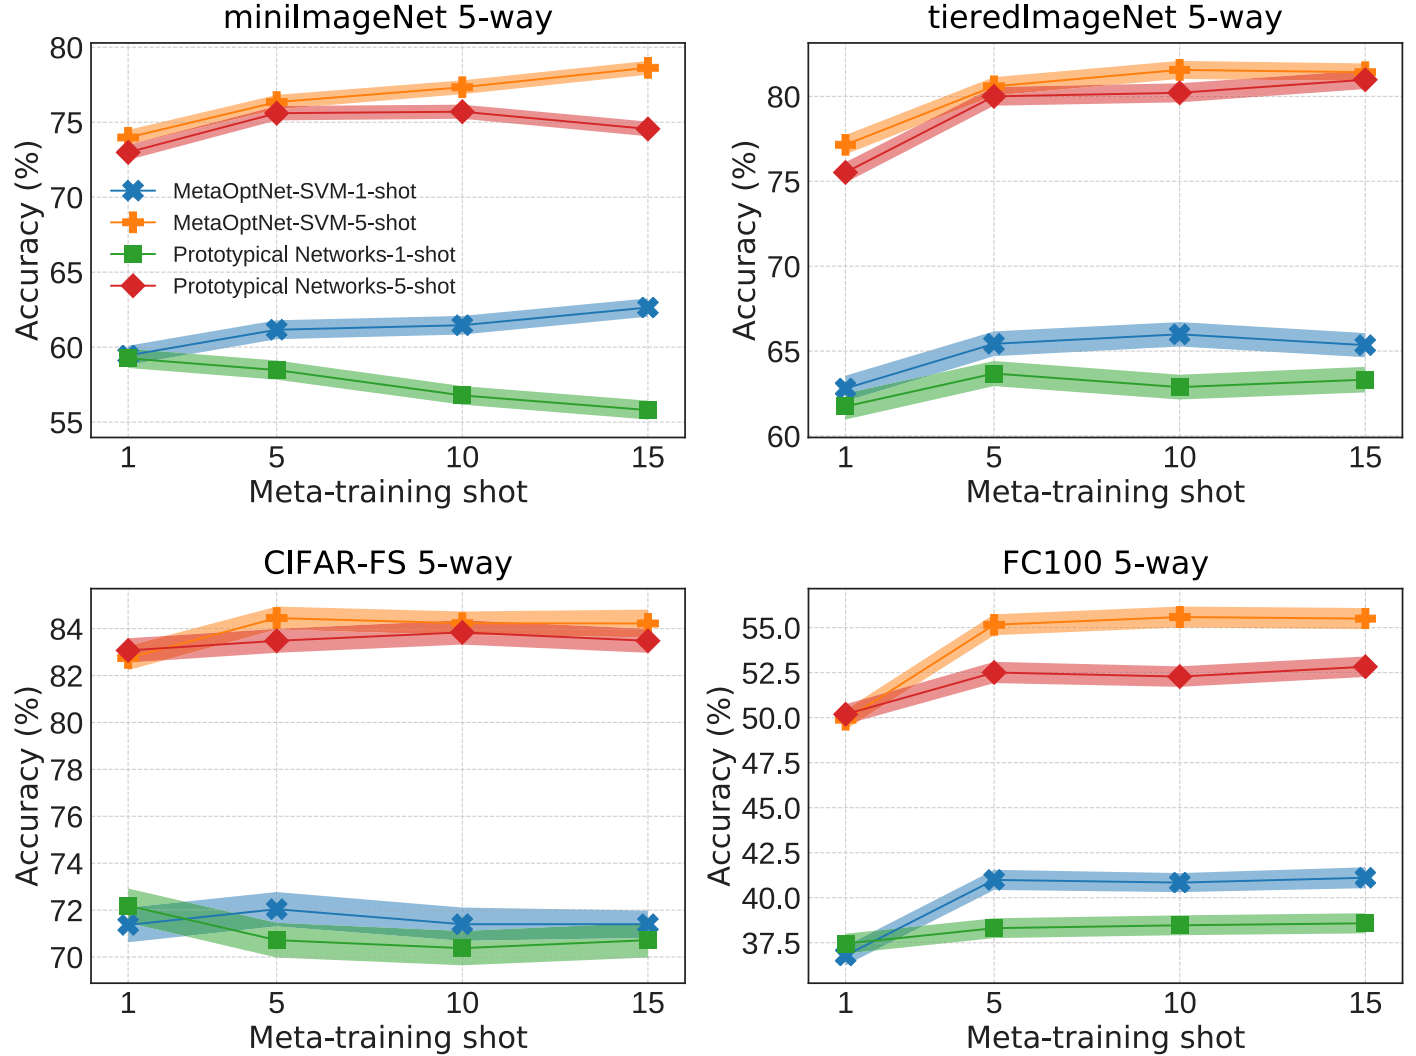
\includegraphics[width=.7\linewidth]{figure/f2.png}
%     \caption{使用不同的元训练样本数量,在miniImageNet元测试集上的测试准确率(\%)。}
%     \label{fig:2}
% \end{figure}

% % 在基学习器的设置方面,对于线性分类器的训练,本文使用二次规划求解器OptNet \upcite{amos2017optnet}。
% % SVM的正则化参数C设置为0.1。岭回归的正则化参数λ设置为50.0。对于最近类均值(原型网络),
% % 本文使用针对特征维度进行归一化的平方欧氏距离。

% % 在提前停止方面,虽然本文可以运行优化器直到收敛,但在实践中,本文发现在固定的迭代次数(仅三次)
% % 内运行QP求解器实际上效果很好。提前停止起到了额外的正则化作用,甚至可以带来稍微更好的性能。


% \subsection{在ImageNet的衍生数据集上的实验}

% miniImageNet数据集\upcite{vinyals2016matching}是用于少样本图像分类的标准基准测试,
% 由ILSVRC-2012 \upcite{russakovsky2015imagenet}中随机选择的100个类组成。
% tieredImageNet基准测试\upcite{ren2018meta}是ILSVRC-2012 \upcite{russakovsky2015imagenet}的一个较大子集,由608个类别组成,分为34个高级类别。

% 表\ref{table:1}总结了5-way miniImageNet和tieredImageNet上的结果。在miniImageNet和tieredImageNet元测试集上,
% 使用95\%置信区间的平均few-shot分类准确率(\%)。“a-b-c-d”表示每个层中具有a,b,c和d个滤波器的4层卷积网络。
% †表示使用元训练集和元验证集的并集来元训练元学习器。“RR”代表岭回归。
% \begin{table}[htbp]
%     \caption{与之前在miniImageNet和tieredImageNet上的工作进行比较}
%     \resizebox{\linewidth}{!}{  
%     \begin{tabular}{
%     l 
%     l 
%     c 
%     c 
%     l 
%     l }
%     \toprule 
%                                                      &                                   & \multicolumn{2}{c}{\textbf{miniImageNet 5-way}}                                                               & \multicolumn{2}{c}{\textbf{tieredImageNet 5-way}}                                                 \\ \cline{3-6} 
%     \textbf{model}                                   & \textbf{backbone}                 & \textbf{1-shot}                                                   & \textbf{5-shot}                                                   & \multicolumn{1}{c}{\textbf{1-shot}} & \multicolumn{1}{c}{\textbf{5-shot}} \\ \hline
%     Meta-Learning LSTM*                              & 64-64-64-64                       & 43.44 ± 0.77                                                      & 60.60 ± 0.71                                                      & -                                                           & -                                                           \\
%     Matching Networks*                               & 64-64-64-64                       & 43.56 ± 0.84                                                      & 55.31 ± 0.73                                                      & -                                   & -                                   \\
%     MAML                                             & 32-32-32-32                       & 48.70 ± 1.84                                                      & 63.11 ± 0.92                                                      & 51.67 ± 1.81                                                & 70.30 ± 1.75                                                \\
%     Prototypical Networks*                           & 64-64-64-64                       & 49.42 ± 0.78                                                      & 68.20 ± 0.66                                                      & 53.31 ± 0.89                                                & 72.69 ± 0.74                                                \\
%     Relation Networks*                               & 64-96-128-256                     & 50.44 ± 0.82                                                      & 65.32 ± 0.70                                                      & 54.48 ± 0.93                                                & 71.32 ± 0.78                                                \\
%     R2D2                                             & 96-192-384-512                    & 51.2 ± 0.6                                                        & 68.8 ± 0.1                                                        & -                                   & -                                   \\
%     Transductive Prop Nets                           & 64-64-64-64                       & 55.51 ± 0.86                                                      & 69.86 ± 0.65                                                      & 59.91 ± 0.94                                                & 73.30 ± 0.75                                                \\
%     SNAIL                                            & ResNet-12                         & 55.71 ± 0.99                                                      & 68.88 ± 0.92                                                      & -                                   & -                                   \\
%     Dynamic Few-shot                                 & 64-64-128-128                     & 56.20 ± 0.86                                                      & 73.00 ± 0.64                                                      & -                                   & -                                   \\
%     AdaResNet                                        & ResNet-12                         & 56.88 ± 0.62                                                      & 71.94 ± 0.57                                                      & -                                   & -                                   \\
%     TADAM                                            & ResNet-12                         & 58.50 ± 0.30                                                      & 76.70 ± 0.30                                                      & -             -                                   \\
%     Activation to Parameter† & WRN-28-10                         & 59.60 ± 0.41                                                      & 73.74 ± 0.19                                                      & -                                   & -                                   \\
%     LEO                                              & WRN-28-10                         & 61.76 ± 0.08                                                      & 77.59 ± 0.12                                                      & 66.33 ± 0.05                                                & 81.44 ± 0.09                                                \\
%     MetaOptNet-RR (ours)                             & ResNet-12 & 61.41 ± 0.61                                                      & 77.88 ± 0.46                                                      & \textbf{65.36 ± 0.71}                                       & \textbf{81.34 ± 0.52}                                       \\
%     MetaOptNet-SVM (ours)                            & ResNet-12                         & 62.64 ± 0.61                                                      & 78.63 ± 0.46                                                      & \textbf{65.99 ± 0.72}                                       & \textbf{81.56 ± 0.53}                                       \\
%     MetaOptNet-SVM-trainval (ours)†                  & ResNet-12                         & \textbf{64.09 ± 0.62} & \textbf{80.00 ± 0.45} & \textbf{65.81 ± 0.74}                                       & \textbf{81.75 ± 0.53}                                       \\
%     \bottomrule
%     \end{tabular}
%     }
%     \label{table:1}
% \end{table}
% 本文的方法在5-way miniImageNet和tieredImageNet基准测试上取得了最先进的性能。
% % 需要注意的是,LEO \upcite{rusu2018meta}除了使用WRN-28-10主干网络外,还利用编码器和关系网络来产生梯度下降的样本相关初始化。
% % TADAM \upcite{oreshkin2018tadam}为每个卷积层使用任务嵌入网络(TEN)块,用于预测元素级比例和偏移向量。

% % 本文还注意到,\upcite{rusu2018meta,qiao2018few}对WRN-28-10特征提取器\upcite{zagoruyko2016wide}进行了预训练,以共同分类miniImageNet元训练集中的全部64个类别;然后在元训练期间冻结网络。
% % \upcite{oreshkin2018tadam}使用了一种类似的策略,使用标准分类任务:他们同时在few-shot分类任务(5-way)和标准分类任务(64-way)上联合训练特征嵌入。
% % 相比之下,
% % 本文的系统是端到端进行元训练的,明确地训练特征提取器在带有正则化线性分类器的few-shot学习任务上表现良好。

% \subsection{CIFAR派生数据集的实验}

% CIFAR-FS数据集\upcite{bertinetto2018meta}是最近提出的few-shot图像分类基准测试,
% 由CIFAR-100 \upcite{krizhevsky2010cifar}中的全部100个类别组成。
% FC100数据集\upcite{oreshkin2018tadam}是另一个源自CIFAR-100 \upcite{krizhevsky2010cifar}的数据集,包含100个类别,这些类别被分成20个超类。

% 表\ref{table:2}总结了5-way分类任务的结果,本文的MetaOptNet-SVM方法实现了最先进的性能。

% \begin{table}[htbp]
%     \caption{在不同的元训练样本量下,CIFAR-FS 和 FC100元测试集的测试准确率(以百分比表示)}
%     \resizebox{\linewidth}{!}{  
%     \begin{tabular}{llcccc}
%     \hline
%                                     &                   & \multicolumn{2}{c}{\textbf{CIFAR-FS 5-way}} & \multicolumn{2}{c}{\textbf{FC100 5-way}}                      \\ \hline
%     \textbf{model}                  & \textbf{backbone} & \textbf{1-shot}      & \textbf{5-shot}      & \textbf{1-shot}     & \textbf{5-shot}                         \\ \hline
%     MAML*                           & 32-32-32-32       & 58.9 ± 1.9           & 71.5 ± 1.0           & -                   & -                                       \\
%     Prototypical Networks*†         & 64-64-64-64       & 55.5 ± 0.7           & 72.0 ± 0.6           & 35.3 ± 0.6          & 48.6 ± 0.6                              \\
%     Relation Networks*              & 64-96-128-256     & 55.0 ± 1.0           & 69.3 ± 0.8           & -                   & -                                       \\
%     R2D2                            & 96-192-384-512    & 65.3 ± 0.2           & 79.4 ± 0.1           & -                   & -                                       \\
%     TADAM                           & ResNet-12         & -                    & -                    & 40.1 ± 0.4          & 56.1 ± 0.4                              \\
%     ProtoNets (our backbone)        & ResNet-12         & \textbf{72.2 ± 0.7}  & 83.5 ± 0.5           & 37.5 ± 0.6          & 52.5 ± 0.6                              \\
%     MetaOptNet-RR (ours)            & ResNet-12         & \textbf{72.6 ± 0.7}  & \textbf{84.3 ± 0.5}  & 40.5 ± 0.6          & 55.3 ± 0.6                              \\
%     MetaOptNet-SVM (ours)           & ResNet-12         & \textbf{72.0 ± 0.7}  & \textbf{84.2 ± 0.5}  & 41.1 ± 0.6          & 55.5 ± 0.6                              \\
%     MetaOptNet-SVM-trainval (ours) & ResNet-12         & \textbf{72.8 ± 0.7}  & \textbf{85.0 ± 0.5}  & \textbf{47.2 ± 0.6} & \multicolumn{1}{l}{\textbf{62.5 ± 0.6}} \\ \hline
%     \end{tabular}
%     }
%     \label{table:2}
% \end{table}

% \section{实验结果比较}

% 表\ref{table:3}显示了本文改变两种不同嵌入架构的基学习器后的结果。当本文使用标准的4层卷积网络,特征维度较低(1600)时,
% 本文没有观察到采用判别式分类器对few-shot学习的实质性益处。事实上,最近邻类均值分类器\upcite{mensink2013distance}在低维特征下表现良好,
% 如Prototypical Networks\upcite{sung2018learning}所示。
% 然而,当嵌入维度远高于16000时,SVM比其他基学习器产生更好的few-shot准确性。因此,当高维特征可用时,正则化线性分类器提供了鲁棒性。

% \begin{table}[htbp]
%     \caption{基础学习器和嵌入网络架构的影响}
%     \resizebox{\linewidth}{!}{  
%     \begin{tabular}{lcccccccc}
%     \hline
%                           & \multicolumn{4}{c}{\textbf{miniImageNet 5-way}}                                    & \multicolumn{4}{c}{\textbf{tieredImageNet 5-way}}                                 \\ \cline{2-9} 
%                           & \multicolumn{2}{c}{\textbf{1-shot}}      & \multicolumn{2}{c}{\textbf{5-shot}}     & \multicolumn{2}{c}{\textbf{1-shot}}     & \multicolumn{2}{c}{\textbf{5-shot}}     \\
%     \textbf{model}        & \textbf{acc. (\%)}  & \textbf{time (ms)} & \textbf{acc. (\%)}  & \textbf{ime (ms)} & \textbf{acc. (\%)}  & \textbf{ime (ms)} & \textbf{acc. (\%)}  & \textbf{ime (ms)} \\ \hline
%     \multicolumn{9}{l}{\textbf{4-layer conv (feature dimension=1600)}}                                                                                                                             \\
%     Prototypical Networks & 53.47±0.63          & 6±0.01             & 70.68±0.49          & 7±0.02            & 54.28±0.67          & 6±0.03            & 71.42±0.61          & 7±0.02            \\
%     MetaOptNet-RR (ours)  & 53.23±0.59          & 20±0.03            & 69.51±0.48          & 27±0.05           & 54.63±0.67          & 21±0.05           & 72.11±0.59          & 28±0.06           \\
%     MetaOptNet-SVM (ours) & 52.87±0.57          & 28±0.02            & 68.76±0.48          & 37±0.05           & 54.71±0.67          & 28±0.07           & 71.79±0.59          & 38±0.08           \\ \hline
%     \multicolumn{9}{l}{\textbf{ResNet-12 (feature dimension=16000)}}                                                                                                                               \\
%     Prototypical Networks & 59.25±0.64          & 60±17              & 75.60±0.48          & 66±17             & 61.74±0.77          & 61±17             & 80.00±0.55          & 66±18             \\
%     MetaOptNet-RR (ours)  & 61.41±0.61          & 68±17              & \textbf{77.88±0.46} & 75±17             & \textbf{65.36±0.71} & 69±17             & \textbf{81.34±0.52} & 77±17             \\
%     MetaOptNet-SVM (ours) & \textbf{62.64±0.61} & 78±17              & \textbf{78.63±0.46} & 89±17             & \textbf{65.99±0.72} & 78±17             & \textbf{81.56±0.53} & 90±17             \\ \hline
%     \end{tabular}
%     }
%     \label{table:3}
%     \end{table}

% % 这种方法的额外好处是计算成本的适度增加。
% 对于ResNet-12,与最近类平均分类器相比,岭回归基学习器的额外开销约为13%,
% SVM基学习器的额外开销约为30-50%。从图\ref{fig:2}可以看出,本文模型的性能在1-shot和5-shot情况下通常随着meta-training shot的增加而增加。
% % 这使得该方法更加实用,因为本文可以使用高shot元训练一次嵌入来适用于所有的meta-testing shot。
% % 本文假设训练数据的类别嵌入比测试数据更紧凑\upcite{yosinski2014transferable},基于此,基学习器的灵活性可以提高对嵌入噪声的鲁棒性并改善泛化能力。

% \section{减少元过拟合}

% % 在元训练结束时,
% % MetaOptNet-SVM与ResNet-12在除tieredImageNet外的所有元训练数据集上几乎都达到了100%的测试准确率。
% 为了缓解过拟合,类似于\upcite{rusu2018meta,qiao2018few},本文使用元训练集和元验证集的并集来元训练嵌入,保持超参数(例如epoch数)与先前设置相同。
% 表\ref{table:1}和表\ref{table:2}显示了使用增强的元训练集(称为MetaOptNet-SVM-trainval)的结果。
% 本文的结果表明,使用更多的元训练“类”进行元学习嵌入有助于减少对元训练集的过拟合。

% 表\ref{table:4}显示了正则化方法对MetaOptNet-SVM与ResNet-12的影响。
% 本文发现如果不使用正则化,则ResNet-12的性能会降低到表\ref{table:3}中每层64个过滤器的4层卷积网络的性能水平。
% 这表明正则化对于元学习非常重要。
% % 本文期望通过引入新的正则化方法,进一步提高少样本学习系统的性能。

% \begin{table}[htbp]
%     \centering
%     \caption{消融研究}
%     \begin{tabular}{ccccc|cc}
%     \hline
%     \textbf{\begin{tabular}[c]{@{}c@{}}Data\\ Aug.\end{tabular}} & \textbf{\begin{tabular}[c]{@{}c@{}}Weight\\ Decay\end{tabular}} & \textbf{\begin{tabular}[c]{@{}c@{}}Drop\\ Block\end{tabular}} & \textbf{\begin{tabular}[c]{@{}c@{}}Label\\ Smt.\end{tabular}} & \textbf{\begin{tabular}[c]{@{}c@{}}Larger\\ Data\end{tabular}} & \textbf{1-shot} & \textbf{5-shot} \\ \hline
%                                                                  & \textbf{}                                                       & \textbf{}                                                     & \textbf{}                                                     & \textbf{}                                                      & 51.13           & 70.88           \\
%     \textbf{√}                                                   & \textbf{}                                                       & \textbf{}                                                     & \textbf{}                                                     & \textbf{}                                                      & 55.80           & 75.76           \\
%     \textbf{}                                                    & \textbf{√}                                                      &                                                               &                                                               &                                                                & 56.65           & 73.72           \\
%     \textbf{√}                                                   & \textbf{√}                                                      &                                                               &                                                               &                                                                & 60.33           & 76.61           \\
%     \textbf{√}                                                   & \textbf{√}                                                      & \textbf{√}                                                    &                                                               &                                                                & 61.11           & 77.40           \\
%     \textbf{√}                                                   & \textbf{√}                                                      & \textbf{√}                                                    & \textbf{√}                                                    &                                                                & 62.64           & 78.63           \\
%     \textbf{√}                                                   & \textbf{√}                                                      & \textbf{√}                                                    & \textbf{√}                                                    & \textbf{√}                                                     & 64.09           & 80.00           \\ \hline
%     \end{tabular}
 
%     \label{table:4}
%     \end{table}

% \section{双重优化效率}

% 为了验证双重优化确实是有效和高效的,本文在 QP 求解器的不同迭代次数下测量了元测试集上的准确性。
% % QP 求解器\upcite{amos2017optnet}的每次迭代都涉及通过 KKT 矩阵的 LU 分解计算原始变量和对偶变量的更新。
% 结果显示在图 \ref{fig:3} 中。QP 求解器在只进行一次迭代的情况下就达到了岭回归目标的最优解。
% 如\upcite{bertinetto2018meta}。此外,本文观察到对于1-shot任务,
% QP SVM求解器在1次迭代中就达到了最优准确率。
% 对于5-shot任务,即使本文只运行一次 QP SVM 求解器,本文也能获得比其他基础学习器更好的准确率。
% % 当 SVM 求解器的迭代次数限制为1次时,一个任务的执行时间为 69±17 毫秒,对于 5-shot 任务是 80±17 毫秒,
% % 这与岭回归求解器的计算成本相当(Table 3)。
% 这些实验表明,在少样本学习的情况下,解决 SVM 和岭回归的对偶目标非常有效。

% \begin{figure}[htbp]
%     \centering
%     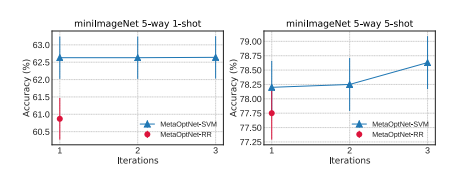
\includegraphics[width=.7\linewidth]{figure/f3.png}
%     \caption{使用不同的元训练样本数量,在miniImageNet元测试集上的测试准确率(\%)。}
%     \label{fig:3}
% \end{figure}
% \endgroup

% \begingroup
% \let\clearpage\relax
% \chapter{结论与展望}

% 本文介绍了一种基于凸基学习器的元学习方法,用于少样本学习。
% 通过利用对偶形式和KKT条件,可以实现计算和内存高效的元学习,
% 特别适用于少样本学习问题。与最近邻分类器相比,
% 线性分类器在适度增加计算成本的情况下提供更好的泛化能力(如表\ref{table:3}所示)。
% 我们的实验表明,正则化线性模型可以在减少过拟合的同时实现显著更高的嵌入维度。

% 未来的研究方向是探索其他凸基学习器,例如核SVM。这将允许更多的训练数据可用于任务,从而逐步增加模型容量的能力。
% \endgroup
\include{data/chapter5-usage}
\include{data/chapter6-implement}
\include{data/conclusion}

% 参考文献
% !Mode:: "TeX:UTF-8"
\cleardoublepage
\phantomsection
\addcontentsline{toc}{chapter}{参考文献}

% [1] Brandon Amos and J. Zico Kolter. OptNet: Differentiable optimization as a layer in neural networks. In ICML, 2017.

% [2] Shane Barratt. On the Differentiability of the Solution to Convex Optimization Problems. arXiv:1804.05098, 2018.

% [3] Luca Bertinetto, Joao F. Henriques, Philip H. S. Torr, and ˜ Andrea Vedaldi. Meta-learning with differentiable closedform solvers. In ICLR, 2019. 2, 4, 5, 6, 7, 8

% [4] Rich Caruana, Nikos Karampatziakis, and Ainur Yessenalina. An empirical evaluation of supervised learning in high dimensions. In ICML, 2008. 1

% [5] Koby Crammer and Yoram Singer. On the algorithmic implementation of multiclass kernel-based vector machines. J. Mach. Learn. Res., 2:265–292, Mar. 2002. 1, 3

% [6] Justin Domke. Generic methods for optimization-based modeling. In AISTATS, 2012. 2

% [7] Asen L. Dontchev and R. Tyrrell Rockafellar. Implicit functions and solution mappings. Springer Monogr. Math., 2009. 4

% [8] Chelsea Finn, Pieter Abbeel, and Sergey Levine. Modelagnostic meta-learning for fast adaptation of deep networks. In ICML, 2017. 1, 2, 3, 6, 7, 8

% [9] Golnaz Ghiasi, Tsung-Yi Lin, and Quoc V. Le. Dropblock: A regularization method for convolutional networks. In NeurIPS, 2018. 5

% [10] Spyros Gidaris and Nikos Komodakis. Dynamic few-shot visual learning without forgetting. In CVPR, 2018. 5, 6

% [11] Stephen Gould, Basura Fernando, Anoop Cherian, Peter Anderson, Rodrigo Santa Cruz, and Edison Guo. On differentiating parameterized argmin and argmax problems with application to bi-level optimization. arXiv preprint arXiv:1607.05447, 2016. 1, 2

% [12] Steven G. Krantz and Harold R. Parks. The implicit function theorem: history, theory, and applications. Springer Science & Business Media, 2012. 2, 4

% [13] Alex Krizhevsky, Vinod Nair, and Geoffrey Hinton. Cifar- 100 (canadian institute for advanced research). 6

% [14] Yanbin Liu, Juho Lee, Minseop Park, Saehoon Kim, and Yi Yang. Transductive propagation network for few-shot learning. In ICLR, 2019. 6

% [15] Dougal Maclaurin, David Duvenaud, and Ryan Adams. Gradient-based hyperparameter optimization through reversible learning. In ICML, 2015. 2

% [16] Tomasz Malisiewicz, Abhinav Gupta, and Alexei A. Efros. Ensemble of exemplar-svms for object detection and beyond. In ICCV, 2011. 1

% [17] Thomas Mensink, Jakob Verbeek, Florent Perronnin, and Gabriella Csurka. Distance-based image classification: Generalizing to new classes at near-zero cost. IEEE Trans. Pattern Anal. Mach. Intell., 35(11):2624–2637, Nov. 2013. 7

% [18] Nikhil Mishra, Mostafa Rohaninejad, Xi Chen, and Pieter Abbeel. A simple neural attentive meta-learner. In ICLR, 2018. 2, 5, 6

% [19] Tsendsuren Munkhdalai, Xingdi Yuan, Soroush Mehri, and Adam Trischler. Rapid adaptation with conditionally shifted neurons. In ICML, 2018. 2, 6

% [20] Boris N. Oreshkin, Pau Rodr´ıguez, and Alexandre Lacoste. Tadam: Task dependent adaptive metric for improved fewshot learning. In NeurIPS, 2018. 2, 5, 6, 7

% [21] Siyuan Qiao, Chenxi Liu, Wei Shen, and Alan L. Yuille. Few-shot image recognition by predicting parameters from activations. In CVPR, 2018. 5, 6, 8

% [22] Sachin Ravi and Hugo Larochelle. Optimization as a model for few-shot learning. In ICLR, 2017. 1, 2, 3, 5, 6

% [23] Mengye Ren, Sachin Ravi, Eleni Triantafillou, Jake Snell, Kevin Swersky, Josh B. Tenenbaum, Hugo Larochelle, and Richard S. Zemel. Meta-learning for semi-supervised fewshot classification. In ICLR, 2018. 2, 5

% [24] Olga Russakovsky, Jia Deng, Hao Su, Jonathan Krause, Sanjeev Satheesh, Sean Ma, Zhiheng Huang, Andrej Karpathy, Aditya Khosla, Michael Bernstein, Alexander C. Berg, and Li Fei-Fei. Imagenet large scale visual recognition challenge. Int. J. Comput. Vision, 115(3):211–252, Dec. 2015. 5

% [25] Andrei A. Rusu, Dushyant Rao, Jakub Sygnowski, Oriol Vinyals, Razvan Pascanu, Simon Osindero, and Raia Hadsell. Meta-learning with latent embedding optimization. In ICLR, 2019. 2, 5, 6, 8

% [26] Jurgen Schmidhuber. Evolutionary principles in selfreferential learning. on learning now to learn: The metameta-meta...-hook. Diploma thesis, Technische Universitat Munchen, Germany, 14 May 1987. 2

% [27] Uwe Schmidt and Stefan Roth. Shrinkage fields for effective image restoration. In CVPR, 2014. 2

% [28] Jake Snell, Kevin Swersky, and Richard S. Zemel. Prototypical networks for few-shot learning. In NIPS, 2017. 1, 2, 3, 4, 5, 6, 7, 8

% [29] Flood Sung, Yongxin Yang, Li Zhang, Tao Xiang, Philip H. S. Torr, and Timothy M. Hospedales. Learning to compare: Relation network for few-shot learning. In CVPR, 2018. 6, 7

% [30] Marshall F. Tappen, Ce Liu, Edward H. Adelson, and William T. Freeman. Learning gaussian conditional random fields for low-level vision. In CVPR, 2007. 2

% [31] Sebastian Thrun. Lifelong Learning Algorithms, pages 181– 209. Springer US, Boston, MA, 1998. 2

% [32] Ricardo Vilalta and Youssef Drissi. A perspective view and survey of meta-learning. Artificial Intelligence Review, 18(2):77–95, Jun 2002. 2

% [33] Oriol Vinyals, Charles Blundell, Timothy Lillicrap, Koray Kavukcuoglu, and Daan Wierstra. Matching networks for one shot learning. In NIPS, 2016. 1, 2, 3, 5, 6, 7

% [34] Jason Weston and Chris Watkins. Support Vector Machines for Multiclass Pattern Recognition. In European Symposium On Artificial Neural Networks, 1999. 3

% [35] Jason Yosinski, Jeff Clune, Yoshua Bengio, and Hod Lipson. How transferable are features in deep neural networks? In NIPS, 2014. 7

% [36] Sergey Zagoruyko and Nikos Komodakis. Wide residual networks. In BMVC, 2016. 6
\nocite{*}
\bibliography{data/bibs}
\cleardoublepage

% 附录
\appendix
% !Mode:: "TeX:UTF-8"
\chapter{参考文献统计}


\begin{table}[htbp]
    \centering
        \begin{tabular}{lcc}
        \hline
        \textbf{作者}             & \multicolumn{1}{l}{\textbf{发文数量}} & \textbf{被引次数} \\ \hline
        Sergey   Levine         & 120                               & 94714         \\
        Pieter   Abbeel         & 105                               & 107734        \\
        Pieter   Abbeel         & 105                               & 107734        \\
        Abhinav   Gupta         & 75                                & 56187         \\
        Chelsea   Finn          & 53                                & 32446         \\
        Wei   Shen              & 45                                & 6988          \\
        Alexei   A. Efros       & 44                                & 105834        \\
        Basura   Fernando       & 39                                & 8664          \\
        Stephen   Gould         & 36                                & 14846         \\
        Kolter                  & 35                                & 25598         \\
        Anoop   Cherian         & 27                                & 3061          \\
        AL   Dontchev           & 22                                & 7479          \\
        Amos                    & 18                                & 6248          \\
        Jakob   Verbeek         & 18                                & 19538         \\
        Pau   Rodríguez         & 17                                & 2764          \\
        Hugo   Larochelle       & 16                                & 70770         \\
        Thomas   Mensink        & 15                                & 9467          \\
        João   F. Henriques     & 14                                & 18489         \\ \hline
        \end{tabular}
    
    \caption{所选文章涉及作者发文数据表}
    \label{table:a}
\end{table}

\begin{table}[htbp]
    \centering
        \begin{tabular}{lcc}
        \hline
        \textbf{作者}             & \multicolumn{1}{l}{\textbf{发文数量}} & \textbf{被引次数} \\ \hline
        David   Duvenaud        & 14                                & 20883         \\
        Siyuan   Qiao           & 14                                & 2649          \\
        Barratt                 & 12                                & 1411          \\
        Quoc   V. Le            & 10                                & 173557        \\
        Xi   Chen               & 10                                & 25972         \\
        Tsendsuren   Munkhdalai & 10                                & 2885          \\
        Chenxi   Liu            & 10                                & 5189          \\
        R   T Rockafellar       & 9                                 & 93877         \\
        Nikos   Komodakis       & 9                                 & 26201         \\
        Bertinetto              & 8                                 & 11038         \\
        Rich   Caruana          & 8                                 & 39978         \\
        Florent   Perronnin     & 7                                 & 28352         \\
        Steven   Krantz         & 6                                 & 16116         \\
        Dougal   Maclaurin      & 6                                 & 9291          \\
        Koby   Crammer          & 5                                 & 20770         \\
        Nikhil   Mishra         & 3                                 & 1714          \\
        Nikos   Karampatziakis  & 2                                 & 2798          \\
        Tsung-Yi   Lin          & 2                                 & 84561         \\
        Spyros   Gidaris        & 2                                 & 6414          \\
        Xingdi   Yuan           & 2                                 & 2528          \\
        Boris   N. Oreshkin     & 2                                 & 3233          \\
        Golnaz   Ghiasi         & 1                                 & 5232          \\
        Tomasz   Malisiewicz    & 1                                 & 6861          \\ \hline
        \end{tabular}
    
    \caption{所选文章涉及作者发文数据表(续)}
\end{table}


\begin{figure}[htbp]
    \centering
    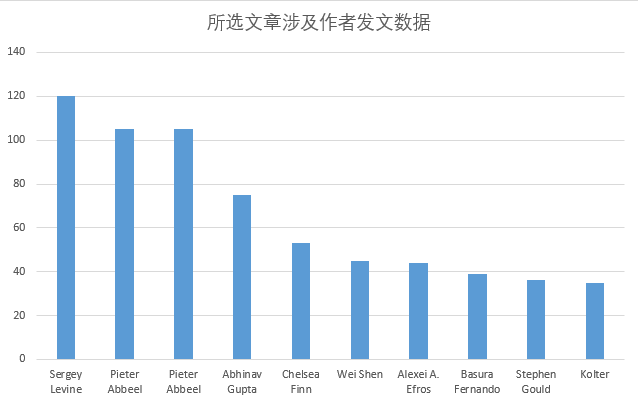
\includegraphics[width=.7\linewidth]{figure/fa.png}
    \caption{所选文章涉及作者发文数据图}
    \label{fig:fa}
\end{figure}

从\ref{table:a} 和 \ref{fig:fa} 中可以看出,发文数量最多的三位作者是Sergey Levine、Pieter Abbeel、Pieter Abbeel。但从\ref{table:a}
可以看出,虽然有些作者发文量不高,但是被引量很高。


\begin{table}[htbp]
    \centering
    \begin{tabular}{lc}
    \hline
    \textbf{国家} & \multicolumn{1}{l}{\textbf{数量}} \\ \hline
    美国          & 12                              \\
    英国          & 2                               \\
    法国          & 2                               \\
    中国          & 2                               \\
    以色列         & 1                               \\
    澳大利亚        & 1                               \\
    加拿大         & 1                               \\ \hline
    \end{tabular}
    \caption{所选文章涉及国家发文数据表}
    \label{table:b}
\end{table}

\begin{figure}[htbp]
    \centering
    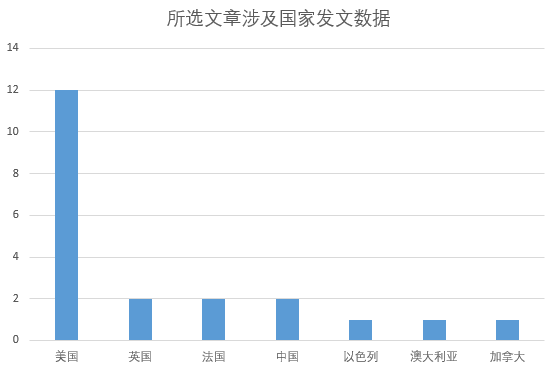
\includegraphics[width=.7\linewidth]{figure/fb.png}
    \caption{所选文章涉及国家发文数据图}
    \label{fig:fb}
\end{figure}

从\ref{table:b} 和 \ref{fig:fb} 可以看出,发文国家最多的是美国,呈现一超多强的格局。

\begin{table}[htbp]
    \centering
    \begin{tabular}{lc}
    \hline
    \textbf{机构}                          & \multicolumn{1}{l}{\textbf{数量}} \\ \hline
    Carnegie Mellon University           & 2                               \\
    University of Oxford                 & 2                               \\
    University of California,   Berkeley & 2                               \\
    Stanford University                  & 1                               \\
    Cornell University                   & 1                               \\
    Hebrew University                    & 1                               \\
    Rochester Institute of   Technology  & 1                               \\
    University of Michigan               & 1                               \\
    University of Washington             & 1                               \\
    google brain                         & 1                               \\
    University Paris-Est                 & 1                               \\
    The   Australian National University & 1                               \\
    Harvard University                   & 1                               \\
    Baidu Research                       & 1                               \\
    INRIA                                & 1                               \\
    Microsoft Research                   & 1                               \\
    Element AI                           & 1                               \\
    Johns Hopkins University             & 1                               \\
    Shanghai University                  & 1                               \\
    Cambridge                            & 1                               \\ \hline
    \end{tabular}
    \caption{所选文章涉及机构发文数据表}
    \label{table:c}
    \end{table}

    \begin{figure}[htbp]
        \centering
        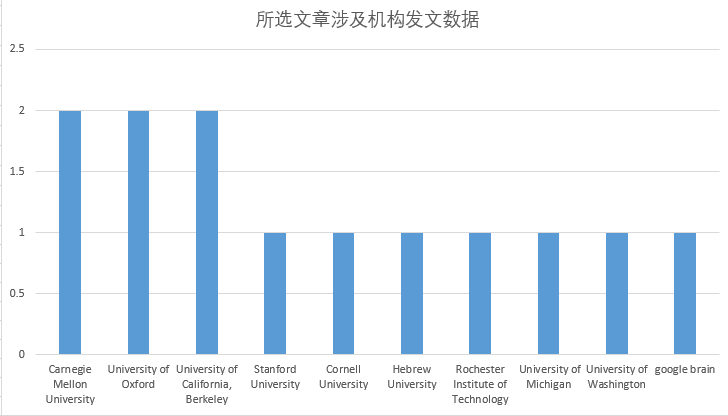
\includegraphics[width=.7\linewidth]{figure/fc.png}
        \caption{所选文章涉及机构发文数据图}
        \label{fig:fc}
    \end{figure}
    
    从\ref{table:c} 和 \ref{fig:fc} 可以看出,发文机构之间差距不大,大多机构是大学,大型科技企业。

    \begin{table}[htbp]
        \centering
        \begin{tabular}{lc}
        \hline
        \textbf{期刊会议}                                       & \textbf{次数} \\ \hline
        ICLR                                                & 6           \\
        PMLR                                                & 5           \\
        ICML                                                & 5           \\
        CVPR                                                & 5           \\
        NIPS                                                & 5           \\
        IEEE                                                & 4           \\
        Advances in neural information   processing systems & 3           \\
        arXiv                                               & 2           \\
        Journal of machine learning   research              & 1           \\
        Artificial intelligence review                      & 1           \\
        Learning to learn                                   & 1           \\
        ICCV                                                & 1           \\
        BMVC                                                & 1          
        \end{tabular}
        \label{table:d}
        \caption{所选文章涉及期刊发文数据表}
    \end{table}

    \begin{figure}[htbp]
        \centering
        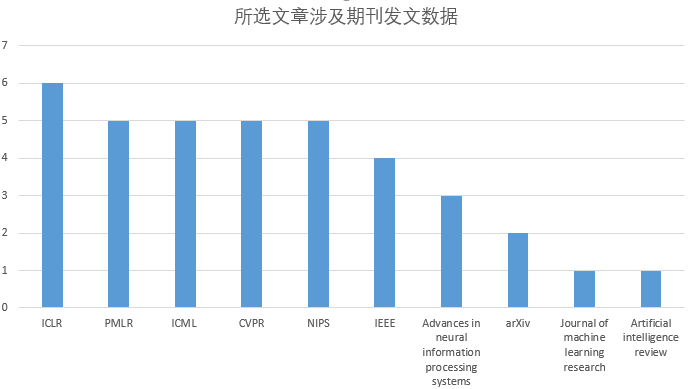
\includegraphics[width=.7\linewidth]{figure/fd.png}
        \caption{所选文章涉及机构发文数据图}
        \label{fig:fd}
    \end{figure}
    
    从\ref{table:d} 和 \ref{fig:fd} 可以看出,在元学习领域内,较为权威的期刊是 ICLR、PMLR、ICML、CVPR、NIPS。
% !Mode:: "TeX:UTF-8"
\chapter{参考文献说明}

\section{第一类}

\cite{amos2017optnet} 该文献是本文采用的主要技术。

\cite{bertinetto2018meta} 该文献是本文采用的主要优化方法。

\cite{bertinetto2018meta} 该文献是本文的主要研究背景和比较对象。

\cite{caruana2008empirical} 该文献是本文的主要研究背景和比较对象。

\cite{crammer2001algorithmic} 该文献是本文的主要研究背景和比较对象。

\section{第二类}

\cite{domke2012generic} 该文献是本文优化方法的相关研究。

\cite{finn2017model} 该文献是本文深度优化方法的相关研究。

\cite{gould2016differentiating} 该文献是本文可微凸优化的相关研究。

\cite{krantz2002implicit} 该文献是一篇相关方向的文献综述。

\cite{maclaurin2015gradient} 该文献与文中采用的算法相关。

\section{第三类}

\cite{malisiewicz2011ensemble} 该文献为本文中采用的基础学习器相关研究。

\cite{mishra2017simple} 该文献为本文之前的在小样本学习领域内重要研究。

\cite{munkhdalai2018rapid} 该文献为本文之前的在小样本学习领域内重要研究。

\cite{oreshkin2018tadam} 该文献为本文之前的在小样本学习领域内重要研究。

\cite{ravi2017optimization} 该文献为本文之前的在小样本学习领域内重要研究。

\cite{ren2018meta} 该文献为本文之前的在小样本学习领域内重要研究。

\cite{rusu2018meta} 该文献为本文之前的在小样本学习领域内重要研究。

\cite{schmidhuber1987evolutionary} 该文献为本文之前的在小样本学习领域内梯度方法的相关研究。

\cite{schmidt2014shrinkage}  该文献为本文研究背景中提到的之前的研究。

\cite{snell2017prototypical} 该文献为本文之前的在小样本学习领域内重要研究。

\cite{tappen2007learning} 本文采用的算法的早期相关研究。

\cite{thrun1998lifelong} 该文献为本文之前的在小样本学习领域研究目标的相关描述。

\cite{vilalta2002perspective} 元学习问题综述。

\cite{vinyals2016matching} 小样本学习问题相关研究。

\end{document}
